\documentclass[border=6pt]{standalone}
\usepackage{tikz}
\usepackage[edges]{forest}
\usetikzlibrary{arrows.meta,positioning,calc,decorations.pathreplacing,shapes.geometric}
\begin{document}
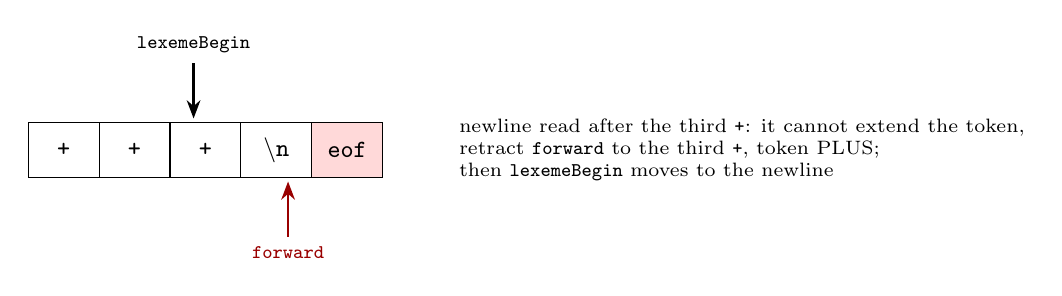
\begin{tikzpicture}[>=Stealth,font=\small,cell/.style={draw,minimum width=0.9cm,minimum height=0.7cm,font=\ttfamily\small}]
\node[cell,fill=white] at (0.00,0) {+};
\node[cell,fill=white] at (0.90,0) {+};
\node[cell,fill=white] at (1.80,0) {+};
\node[cell,fill=white] at (2.70,0) {\textbackslash n};
\node[cell,fill=red!15] at (3.60,0) {eof};
\draw[->,thick] (1.65,1.1) node[above,font=\scriptsize\ttfamily]{lexemeBegin} -- (1.65,0.4);
\draw[->,thick,red!60!black] (2.85,-1.1) node[below,font=\scriptsize\ttfamily]{forward} -- (2.85,-0.4);
\node[font=\scriptsize,anchor=west,align=left] at (4.9,0) {newline read after the third \texttt{+}: it cannot extend the token,\\retract \texttt{forward} to the third \texttt{+}, token PLUS;\\then \texttt{lexemeBegin} moves to the newline};
\end{tikzpicture}
\end{document}
